\hoofdstuk{Mobile platforms}



\paragraaf{Introduction}
% per platform: van wie is het, wat is de geschiedenis, waar wordt het gebruikt, welke achterliggende techniek drijft het?
% plaatjes homescreens of devices toevoegen, visueel maken.

In order to define which mobile platforms should be targeted for cross-platform mobile application development the following chapter presents a concise overview of:

\begin{itemize}
\item
the current mobile operating systems for mobile platforms, with in smartphones specific. 
\item
the current market share and trends
\end{itemize}

In this thesis \emph{mobile platforms} encapsulate only smartphones as it has not been a requirement to support tablets and other mobile devices.

A smartphone can be defined as a smart phone is a next-generation, multifunctional cell phone that provides voice communication and text-messaging capabilities and facilitates data processing as well as enhanced wireless connectivity.\cite{Ni2006}



\subparagraaf{Apple iOS}
iOS is a proprietary mobile operating system, developed by Apple Inc. It was originally released in 2007 for the iPhone and iPod Touch. iOS also became the main operating system of the iPad and Apple TV.

\begin{centering}
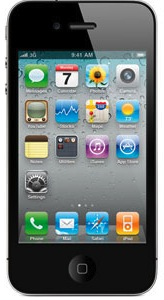
\includegraphics[scale=0.5]{images/iphone4.jpg}\\{4th generation Apple iPhone running iOS 4}\\
\end{centering}


\subparagraaf{Google Android}
Android is a open source mobile operating system, developed by the Open Handset Alliance, led by Google and other companies.\cite{Inc.2012}

\begin{centering}
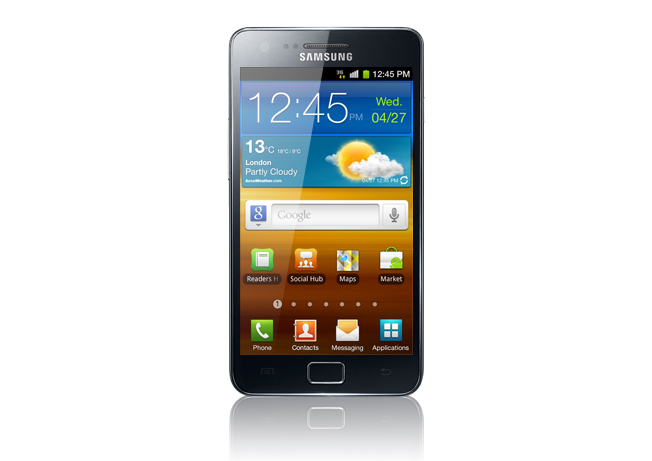
\includegraphics[scale=0.35]{images/android_sgs2.jpg}\\{Samsung Galaxy S2 running Android 2.3}\\
\end{centering}


\subparagraaf{BlackBerry OS}
BlackBerry OS is a proprietary mobile operating system, developed by RIM\emph{(Research In Motion)} for its line of BlackBerry mobile devices.

\begin{centering}
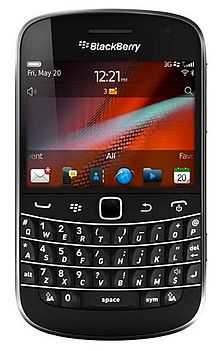
\includegraphics[scale=0.5]{images/Blackberrybold9900.jpg}\\{BlackBerry Bold 9900 running BlackBerry OS 7.1}\\
\end{centering}


\subparagraaf{Windows Phone 7}
Windows Phone 7 is a mobile operating system developed by Microsoft as a successor to its Windows Mobile platform.

\begin{centering}
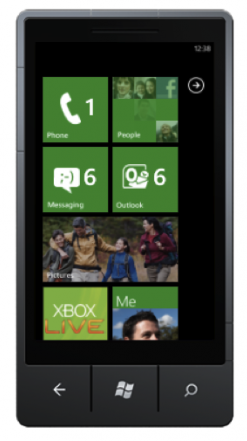
\includegraphics[scale=0.35]{images/WindowsPhone7.png}\\{Windows Phone 7}\\
\end{centering}


\subparagraaf{Other platforms}
% Onder other valt Symbian. Symbian is een app platforms dus we nemen het mee:)
\subparagraaf{Java ME}
\subparagraaf{Symbian}

\paragraaf{Distribution of applications}
%todo

\paragraaf{Market share and trend}
% TODO: waar de stats vandaan komen,  wat ze betekenen, waarom ik ze heb gekozen, wat de alternatieven zijn((gartner 2011)\
% platform specifiek maken: smartphone only? want daar focussen we op.

\begin{centering}
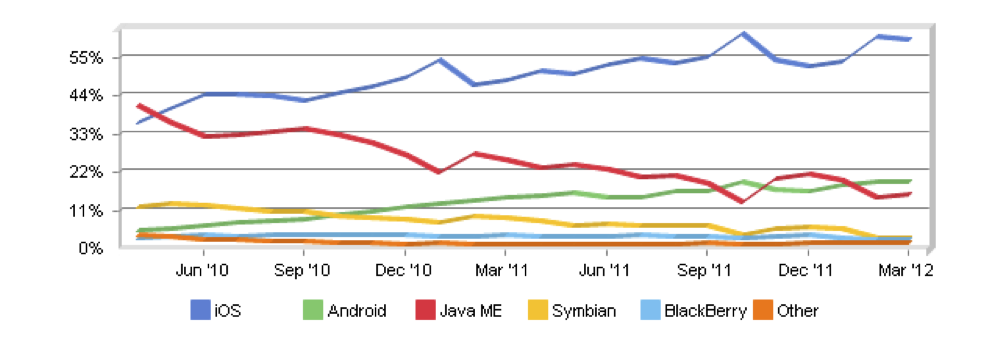
\includegraphics[scale=0.5]{images/marketsharetrendsApril10Tomay12.png}\\{World wide mobile OS Marketshare trends, April 2010 up to may 2012}\\
\end{centering}

\begin{centering}
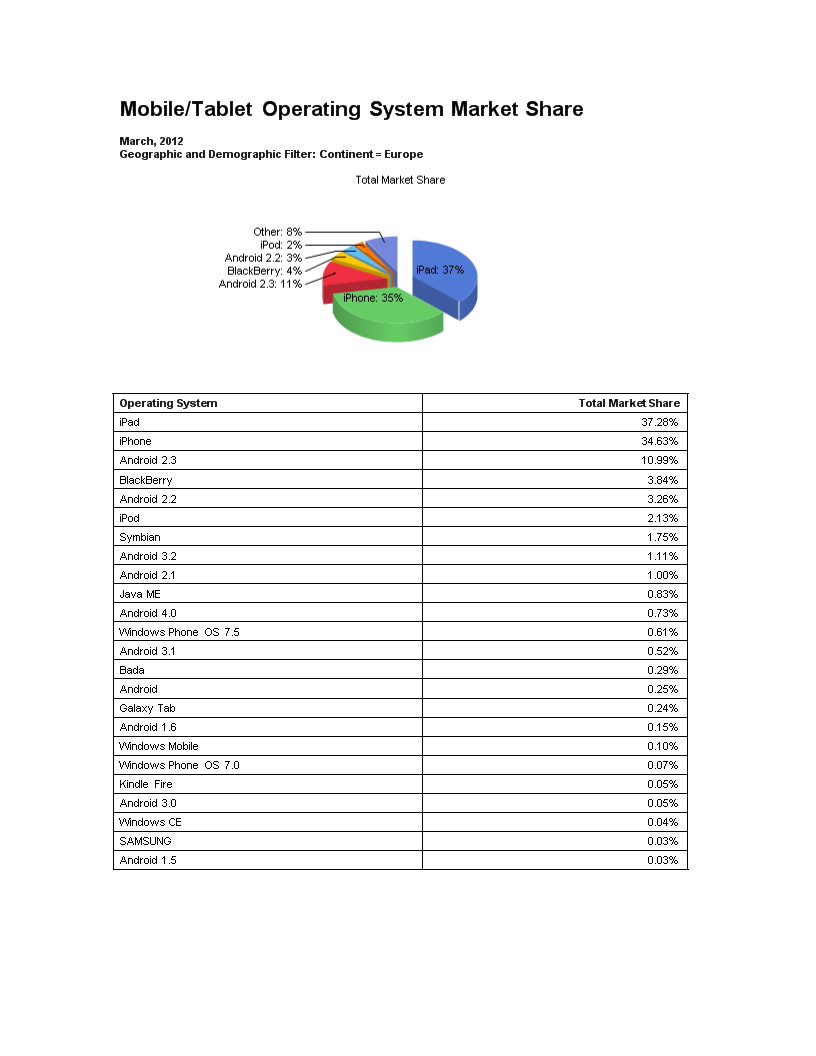
\includegraphics[scale=0.5]{images/netmarketshare_march2012.png}\\
\end{centering}

\begin{tabel}{|>\R p{\Procent{25}} | >\R p{\Procent{25}} |}{vbx}{Market share in the european continent as of march 2012\cite{Netmarketshare2012}}
\hline
\bf{Operating System} & \bf{Total \% Market Share}\\
\hline \hline
iOS & 74.04\\
Android & 18.36\\
BlackBerry & 3.84\\
Symbian & 1.75\\
Java ME & 0.83\\
Windows Phone & 0.68\\
Bada & 0.29\\
Windows Mobile & 0.14\\
Kindle & 0.05\\
Samsung & 0.03\\
LG & 0.01\\
ZTE & 0.00\\
Palm & 0.00\\
\hline
\end{tabel}

\paragraaf{Conclusion}
%vertellen waarom Android en iOS getarget worden: marketshare + trend koppelen aan een requirement van Lunatech

